\documentclass[preprint, 3p,
authoryear]{elsarticle} %review=doublespace preprint=single 5p=2 column
%%% Begin My package additions %%%%%%%%%%%%%%%%%%%

\usepackage[hyphens]{url}

  \journal{Some Journal} % Sets Journal name

\usepackage{graphicx}
%%%%%%%%%%%%%%%% end my additions to header

\usepackage[T1]{fontenc}
\usepackage{lmodern}
\usepackage{amssymb,amsmath}
% TODO: Currently lineno needs to be loaded after amsmath because of conflict
% https://github.com/latex-lineno/lineno/issues/5
\usepackage{lineno} % add
\usepackage{ifxetex,ifluatex}
\usepackage{fixltx2e} % provides \textsubscript
% use upquote if available, for straight quotes in verbatim environments
\IfFileExists{upquote.sty}{\usepackage{upquote}}{}
\ifnum 0\ifxetex 1\fi\ifluatex 1\fi=0 % if pdftex
  \usepackage[utf8]{inputenc}
\else % if luatex or xelatex
  \usepackage{fontspec}
  \ifxetex
    \usepackage{xltxtra,xunicode}
  \fi
  \defaultfontfeatures{Mapping=tex-text,Scale=MatchLowercase}
  \newcommand{\euro}{€}
\fi
% use microtype if available
\IfFileExists{microtype.sty}{\usepackage{microtype}}{}
\usepackage[]{natbib}
\bibliographystyle{plainnat}

\ifxetex
  \usepackage[setpagesize=false, % page size defined by xetex
              unicode=false, % unicode breaks when used with xetex
              xetex]{hyperref}
\else
  \usepackage[unicode=true]{hyperref}
\fi
\hypersetup{breaklinks=true,
            bookmarks=true,
            pdfauthor={},
            pdftitle={Course Project - BIOL520I - Mock Manuscript},
            colorlinks=false,
            urlcolor=blue,
            linkcolor=magenta,
            pdfborder={0 0 0}}

\setcounter{secnumdepth}{5}
% Pandoc toggle for numbering sections (defaults to be off)


% tightlist command for lists without linebreak
\providecommand{\tightlist}{%
  \setlength{\itemsep}{0pt}\setlength{\parskip}{0pt}}

% From pandoc table feature
\usepackage{longtable,booktabs,array}
\usepackage{calc} % for calculating minipage widths
% Correct order of tables after \paragraph or \subparagraph
\usepackage{etoolbox}
\makeatletter
\patchcmd\longtable{\par}{\if@noskipsec\mbox{}\fi\par}{}{}
\makeatother
% Allow footnotes in longtable head/foot
\IfFileExists{footnotehyper.sty}{\usepackage{footnotehyper}}{\usepackage{footnote}}
\makesavenoteenv{longtable}






\begin{document}


\begin{frontmatter}

  \title{Course Project - BIOL520I - Mock Manuscript}
    \author[UBC Okanagan]{Harry Zhang%
  \corref{cor1}%
  }
   \ead{harry.zhang@alumni.ubc.ca} 
      \affiliation[UBC Okanagan]{
    organization={University of British Columbia},addressline={100 some
street},city={Kelowna},postcode={123456},state={B.C.},country={Canada},}
    \cortext[cor1]{Corresponding author}
  
  \begin{abstract}
  This is a mock manuscript for course project BIOL520I Productivity and
  Reproducebility. This mini project explores penguin bill attributes in
  data package \emph{palmerpenguins}.
  \end{abstract}
    \begin{keyword}
    mock\_project \sep 
    course\_project
  \end{keyword}
  
 \end{frontmatter}

\hypertarget{introduction}{%
\section{Introduction}\label{introduction}}

In this mini project for course BIOL520I Productivity and
Reproducibility in Ecology and Evolution, the \emph{palmerpenguins} data
package was explored in R to understand the bill attributes of sampled
penguin species. Tables and figures were created in this process. No
in-depth analysis was conducted because the overall purpose of this mini
project is to simply demonstrate a reproducible workflow.

\hypertarget{method}{%
\section{Method}\label{method}}

\hypertarget{data}{%
\subsection{Data}\label{data}}

The dataset used in this project is accessed from R data pacakge
\emph{palmerpenguins} \citep{Horst2020}, originally published in
\citet{Gorman2014}.

\hypertarget{process}{%
\subsection{Process}\label{process}}

The dataset \emph{penguins} was imported to dataframe from the data
package. A copy of the raw, unaltered data was saved as a CSV file. The
dataframe was then examined to understand the data structure
completeness, where observations with missing bill attributes were
dropped for simplicity in this demonstration. After cleaning up the
data, I calculated simple descriptive statistics for bill dimensions
(\emph{bill\_length\_mm} and \emph{bill\_depth\_mm} variables) and
compared them across the three sampled species. Tables and boxplots were
created to show these differences in bill dimensions. An additional
histogram was created to show bill length distribution within the
species \emph{``Adelie''}. Finally, a scatterplot of bill dimensions was
created across all three species with bill length on the x-axis and bill
depth on the y-axis to visualize any potential correlation between the
two variables. The scatter points were colored by species to aid
identification of specific clustering in the variable space.

\hypertarget{results}{%
\section{Results}\label{results}}

The bill lengths by species is summarized in Table \ref{billLen}

\begin{longtable}[]{@{}lrrrr@{}}
\caption{\label{billLen}Bill Length by Species}\tabularnewline
\toprule()
species & min & mean & median & max \\
\midrule()
\endfirsthead
\toprule()
species & min & mean & median & max \\
\midrule()
\endhead
Adelie & 32.1 & 38.79139 & 38.80 & 46.0 \\
Gentoo & 40.9 & 47.50488 & 47.30 & 59.6 \\
Chinstrap & 40.9 & 48.83382 & 49.55 & 58.0 \\
\bottomrule()
\end{longtable}

The bill dimensions scatterplot (Figure \ref{scatter}) shows a visually
detectable positive correlation between \emph{bill\_length\_mm} and
\emph{bill\_depth\_mm} within species. There is specific clustering in
the variable space.

\begin{figure}

{\centering 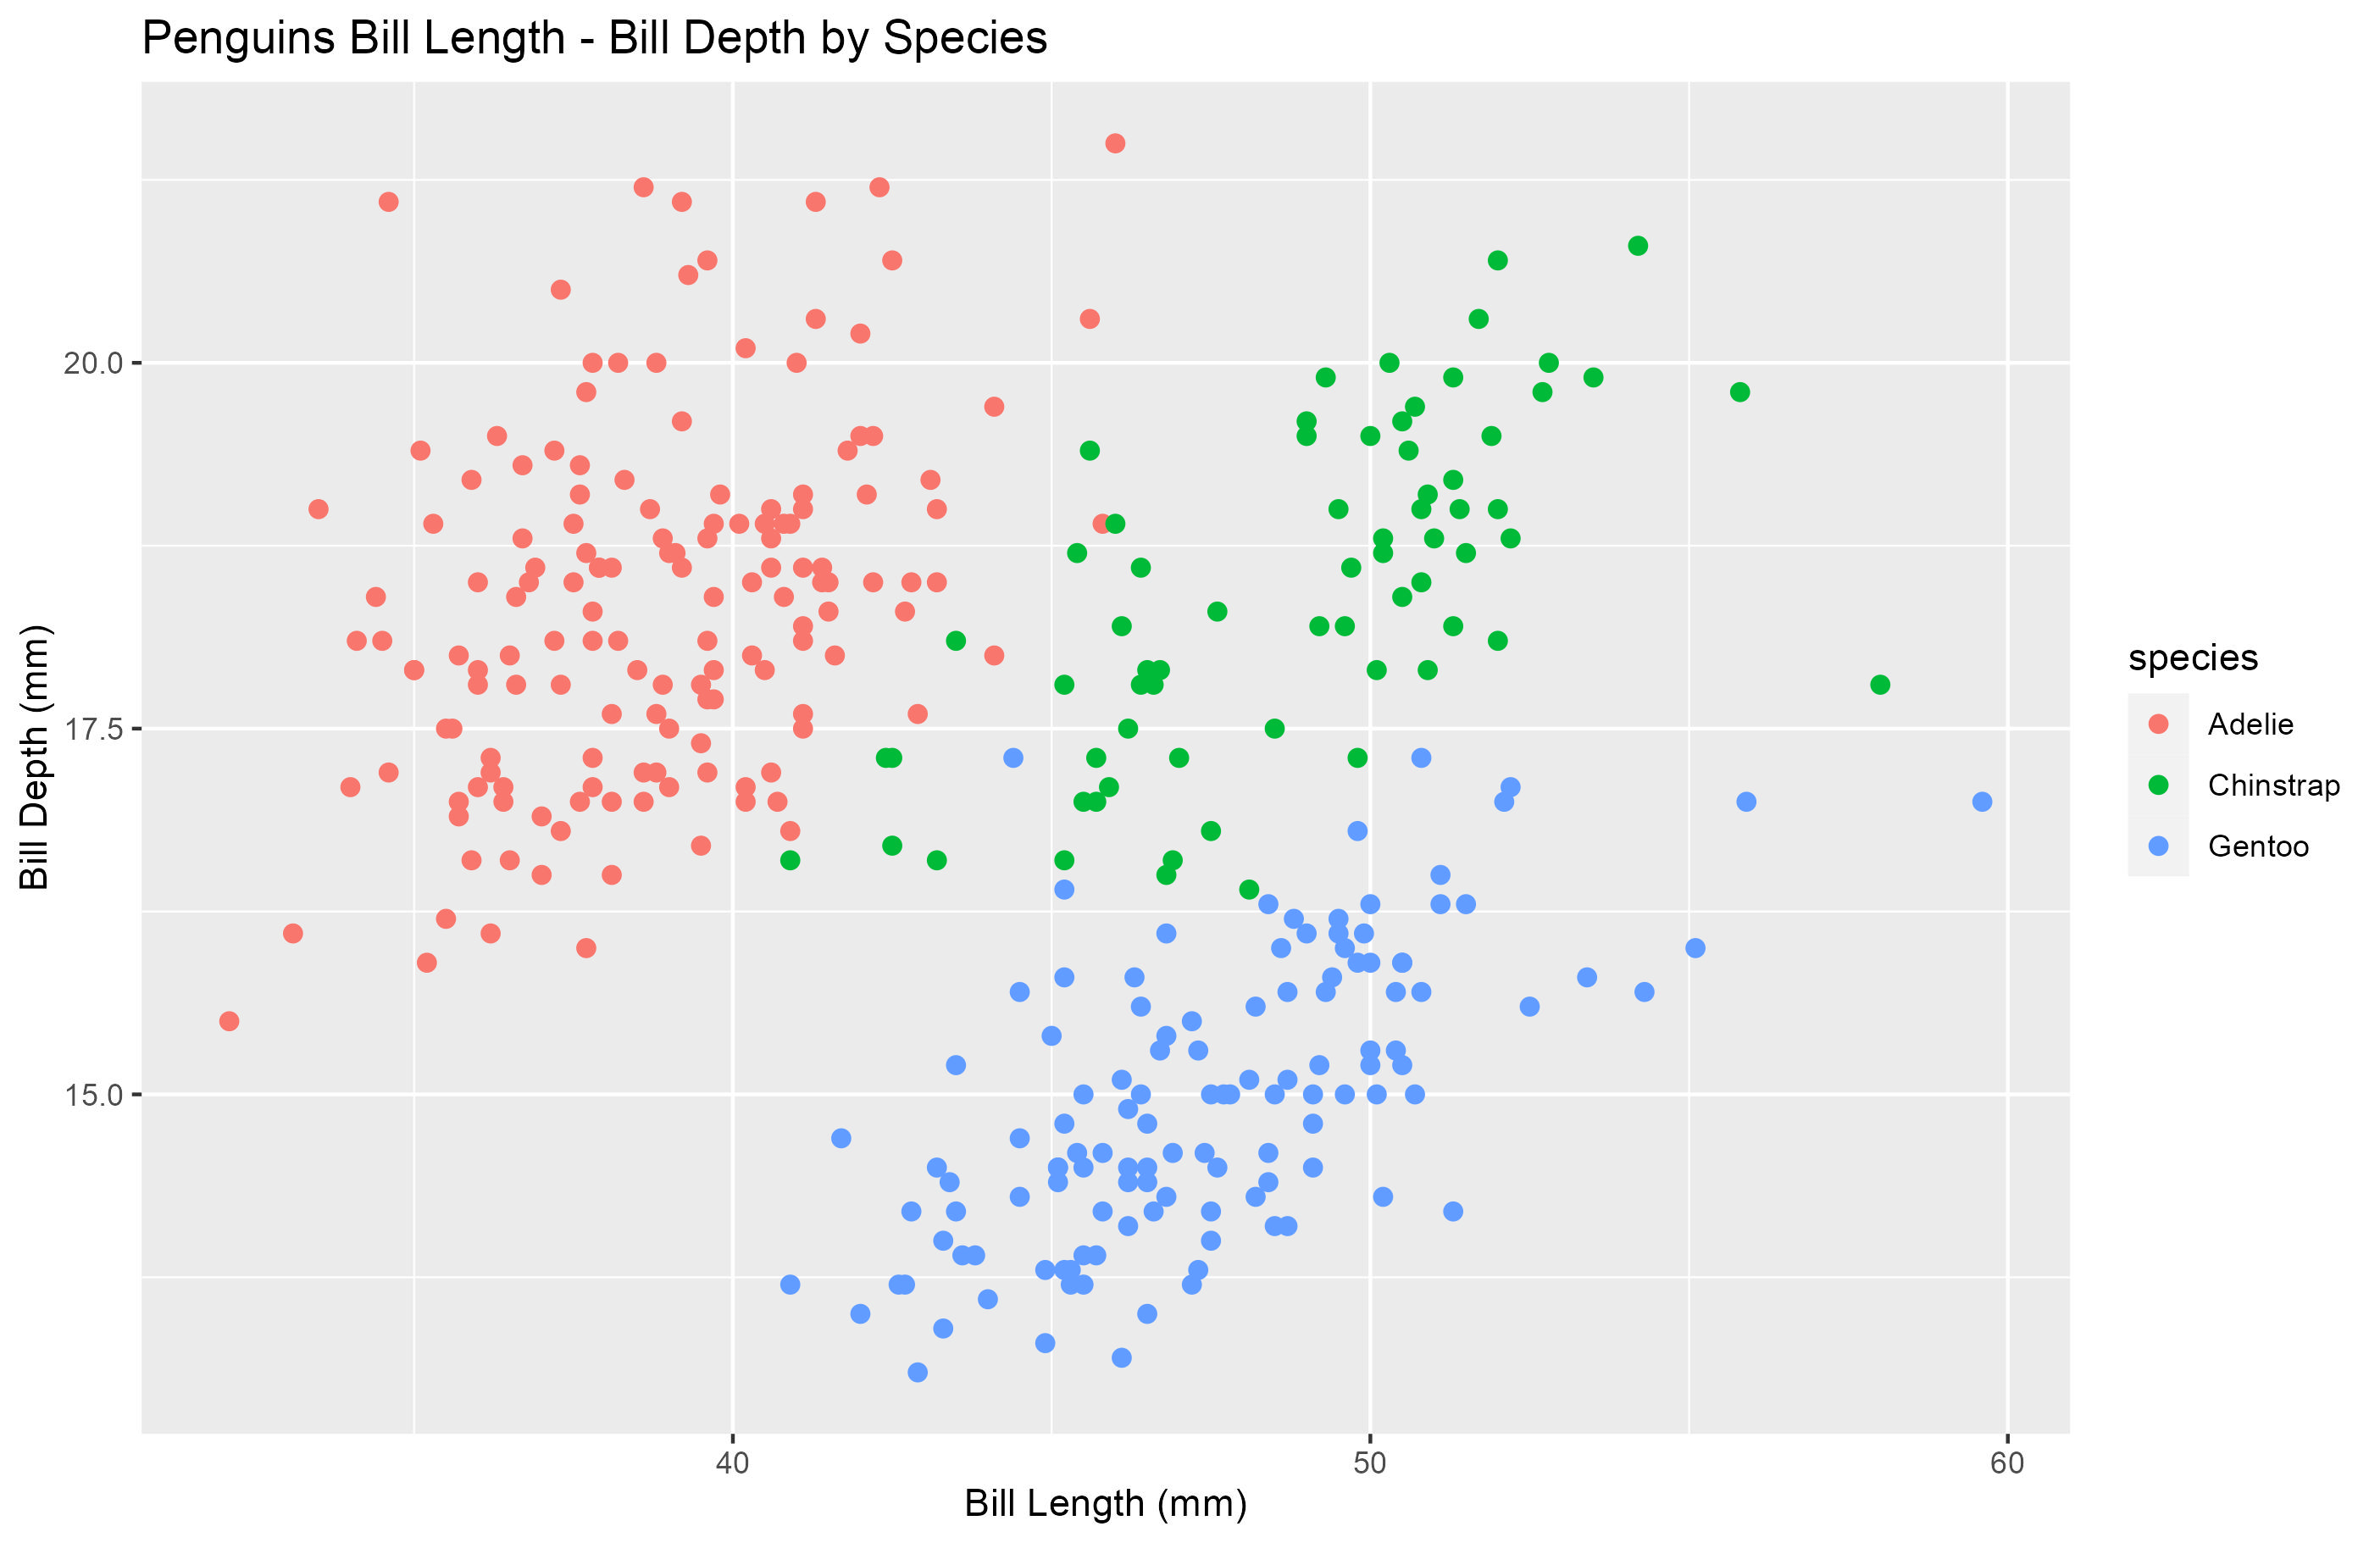
\includegraphics[width=1\linewidth]{../Figures/scatterplot_billLenDep} 

}

\caption{\label{scatter}Scatterplot of Bill Length vs Bill Depth}\label{fig:scatter}
\end{figure}

\hypertarget{discussion}{%
\section{Discussion}\label{discussion}}

I have found a qualitatively positive correlation between bill length
and bill depth in all three sampled penguin species. This correlation
can be quantified using regression methods in future studies.

The bill attribute observations show a tendency of clustering by species
in the bill dimension variable space. This suggests differences in bill
sizes and shape characteristics across the three species. Further
research on these characteristics may lead to quantitative methods to
identify sample species using bill dimension measurements. \pagebreak \#
References \{.unnumbered\}

\bibliography{mybibfile.bib}


\end{document}
